\documentclass{beamer}

\mode<presentation> {
\usetheme{Madrid}
% \usetheme{default}
% \usetheme{PaloAlto}
% \usetheme{EastLansing}
}

\beamertemplatenavigationsymbolsempty

% pacman.sty does not allow numbering pages properly with backup/appendix slides
% \usepackage{pacman}

\usepackage{graphicx} % Allows to include figures
% \usepackage{booktabs} % Allows the use of \toprule, \midrule and \bottomrule in tables
% \usepackage[utf8]{inputenc}
% \usepackage{float}
% \usepackage{mathtools}
% \usepackage{xcolor}
% \usepackage{bm}
% \usepackage{scalerel}
% \usepackage{setspace}
\usepackage{appendixnumberbeamer} % add \appendix

% \usepackage{amsmath}
% \usepackage{amssymb}
\usepackage{mathtools, nccmath}
% \usepackage[mathscr]{euscript}  % euler script font
% \usepackage{cleveref}
% \usepackage{enumitem}

\usepackage{algorithm}
\usepackage[noend]{algpseudocode}

\DeclareMathOperator{\Var}{Var}
\DeclareMathOperator{\modexp}{mod\_exp}
\DeclareMathOperator{\decryptiontime}{decryption\_time}
\DeclareMathOperator{\extrareduction}{extra\ reduction}

\newcommand{\myDegree}{Master of Science Degree in Computer Science}
\newcommand{\myName}{Lorenzo Palloni}
\newcommand{\mySupervisor}{Marco Bertini}
\newcommand{\myFirstCosupervisor}{Leonardo Galteri}
\newcommand{\mySecondCosupervisor}{Donatella Merlini}
\newcommand{\myFaculty}{\protect{School of Mathematics, Physics and Natural Science}}
\newcommand{\myUni}{\protect{University of Florence}}

%---------------------------------------------------------------------------------------
%	TITLE PAGE
%---------------------------------------------------------------------------------------
\title[]{Optimization Techniques of Deep Learning Models for Visual Quality Improvement}


\author{
  \myName
}
\institute[]{
  \includegraphics[scale=0.075]{../thesis/static/logo/LOGO}\\
  % \myUni\\
  \myFaculty\\
  \myDegree\\
  \medskip
  Supervisor: \mySupervisor\\
  Co-supervisor: \myFirstCosupervisor\\
  Co-supervisor: \mySecondCosupervisor
}

\date{April 21, 2023}

\begin{document}

\begin{frame}
  \titlepage % Print the title page as the first slide
\end{frame}
%---------------------------------------------------------------------------------------

%---------------------------------------------------------------------------------------
% TABLE OF CONTENTS
%---------------------------------------------------------------------------------------
%\begin{frame}
%\tableofcontents
%\end{frame}
%---------------------------------------------------------------------------------------

%---------------------------------------------------------------------------------------
\begin{frame}{Introduction}
\begin{itemize}
  \item \textbf{Goal:} Improve video restoration with deep learning models
  \item \textbf{Challenge:} Computational complexity of deep learning models
  \item \textbf{Solution:} Apply quantization techniques for faster inference and reduced memory usage
  \item \textbf{Focus:} Artefact removal and super-resolution tasks
  \item \textbf{Method:} Post-training quantization using TensorRT
  \item \textbf{Impact:} Enable practical deployment on resource-constrained devices
\end{itemize}
\end{frame}
%---------------------------------------------------------------------------------------
%---------------------------------------------------------------------------------------
\begin{frame}{Quality Metrics for Video Restoration}
\begin{itemize}
  \item \textbf{Traditional Metrics:}
  \begin{itemize}
    \item PSNR, MSE, SSIM, MS-SSIM
    \item Simple numerical comparisons
    \item May not correlate well with human perception
  \end{itemize}
  \item \textbf{Perceptual Metrics:}
  \begin{itemize}
    \item FID, LPIPS, LPIPS-Comp, E-LPIPS, DISTS, MOS, 2AFC, JND
    \item Evaluate image quality based on human perception
    \item More complex to compute, but better correlation with perception
  \end{itemize}
  \item \textbf{No-Reference Metrics:}
  \begin{itemize}
    \item BRISQUE, NIQE, PIQUE, CONTRIQUE
    \item Assess image quality without reference images
  \end{itemize}
  \item \textbf{Video Quality Metrics:}
  \begin{itemize}
    \item VMAF
    \item Takes into account temporal aspects of quality degradation
  \end{itemize}
  \end{itemize}
\end{frame}
%---------------------------------------------------------------------------------------
%---------------------------------------------------------------------------------------
\begin{frame}{Architectures}
\begin{itemize}
  \item Overview of UNet and SRUNet model architectures
  \item UNet: encoder-decoder structure with skip connections
  \item SRUNet: modified UNet for super-resolution and artefact removal
  \item Training setup: Generative Adversarial Network (GAN) framework
  \item Generator loss: combination of LPIPS and SSIM metrics
\end{itemize}
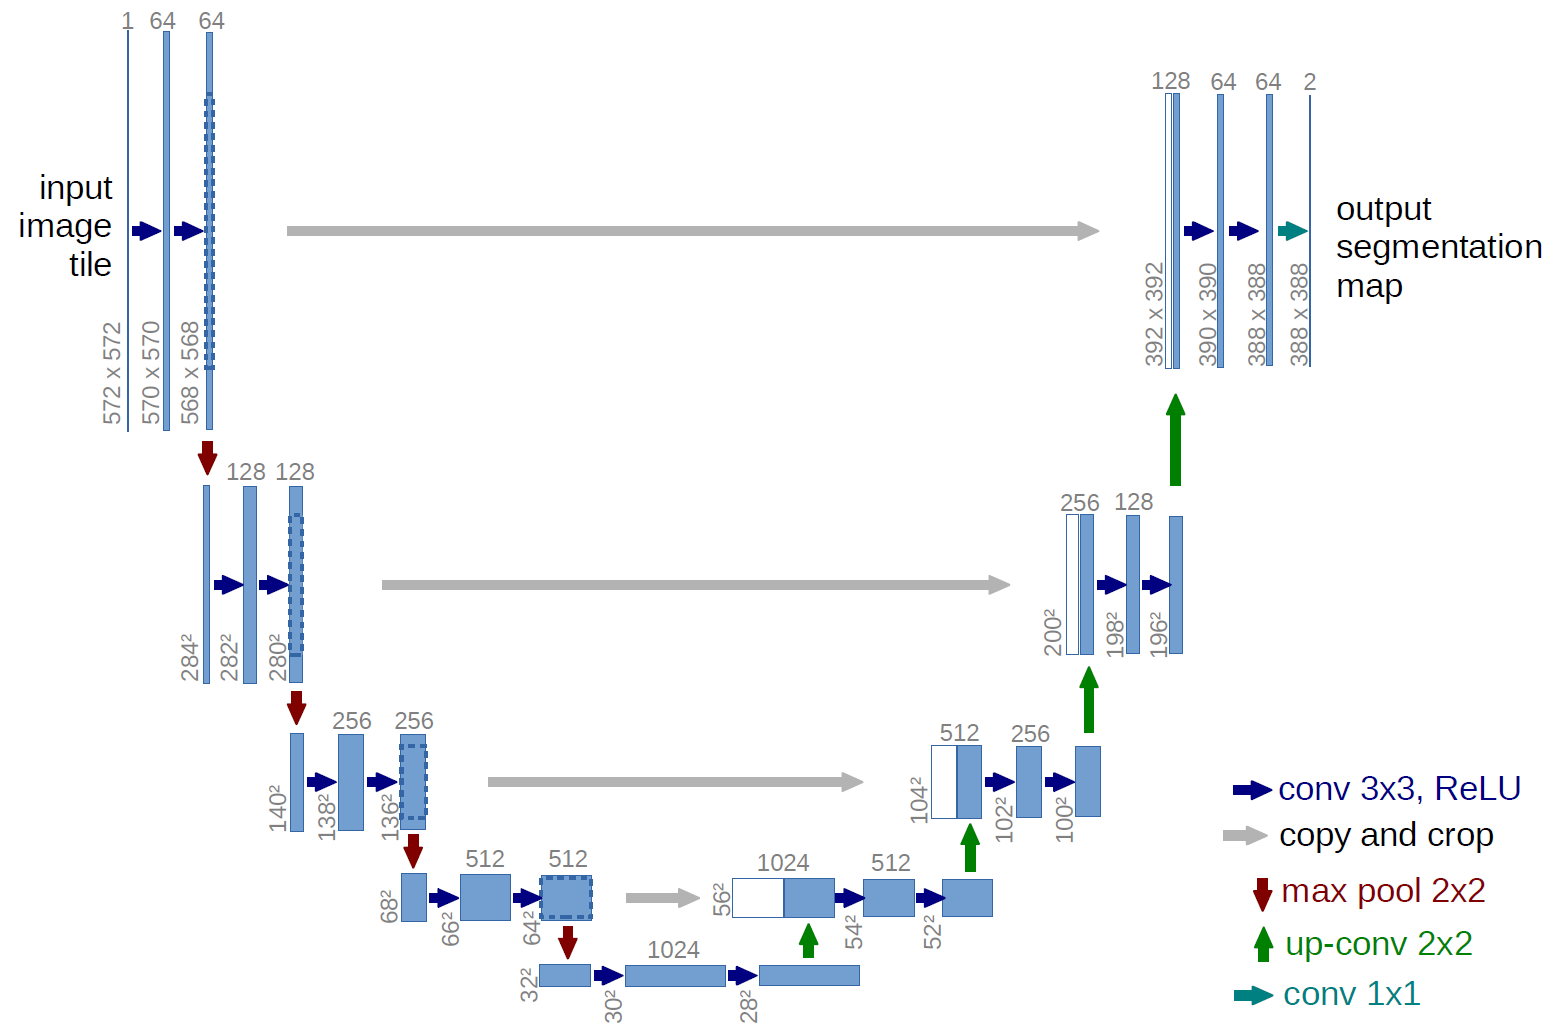
\includegraphics[width=0.45\textwidth]{../thesis/static/unet_architecture.png}
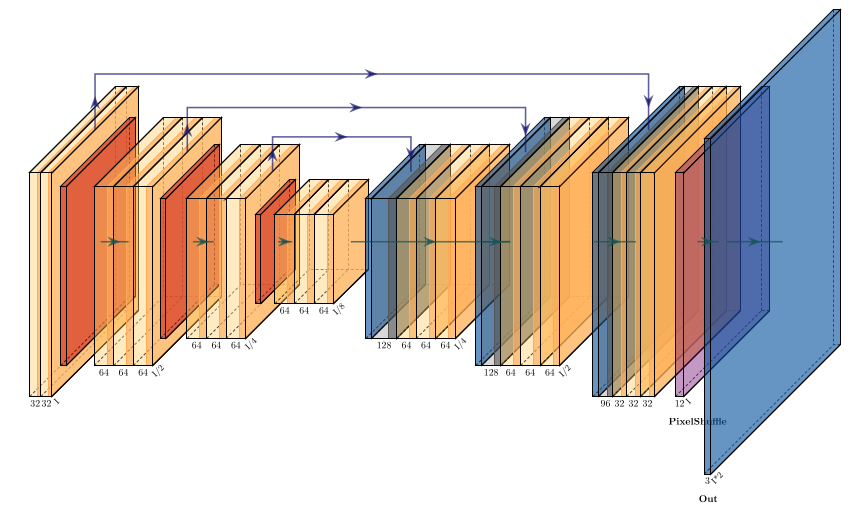
\includegraphics[width=0.45\textwidth]{../thesis/static/srunet_architecture.png}
\end{frame}
%---------------------------------------------------------------------------------------
%---------------------------------------------------------------------------------------
\begin{frame}{Optimizations}
\begin{itemize}
  \item Enhancing deep learning models for super-resolution and visual artefact removal
  \item Factors: architecture, loss functions, evaluation metrics, model weights, hyperparameters
  \item Regularization techniques: dropout and data augmentation
  \item Quantization: reduces memory footprint and computation requirements
  \begin{itemize}
    \item Uniform and non-uniform quantization
    \item Fixed-point, integer, and hybrid quantization
    \item Quantization-Aware Training (QAT) vs Post-Training Quantization (PTQ)
  \end{itemize}
  \item TensorRT: NVIDIA tool to speed up inference
  \item Custom data-loading pipeline: efficient training without GPU bottlenecks
\end{itemize}
\end{frame}
%---------------------------------------------------------------------------------------
%---------------------------------------------------------------------------------------
\begin{frame}{Experiments}
\begin{itemize}
  \item Performance comparison of UNet and SRUNet models.
  \item TensorRT optimization with different precisions: FP32, FP16, and INT8.
  \item Quantitative results: Perceptual and traditional metrics show minor differences between optimized and non-optimized models.
  \item Speedup: Up to 2.38X for UNet and 2.27X for SRUNet using INT8 optimization.
  \item Memory consumption reduced up to 63.3\% for UNet and 53.8\% for SRUNet.
\end{itemize}
\end{frame}
%---------------------------------------------------------------------------------------

% %---------------------------------------------------------------------------------------
% \begin{frame}{Experiments Overview}
% \begin{itemize}
% \item Comparison of UNet and SRUNet models with TensorRT-optimized versions (FP32, FP16, INT8)
% \item Evaluation on 60 test frames using perceptual and traditional metrics
% \item Analysis of inference speed and memory consumption
% \end{itemize}
% \end{frame}
% %---------------------------------------------------------------------------------------

%---------------------------------------------------------------------------------------
\begin{frame}{Quantitative Results: Boxplots of Metrics}
\begin{columns}
\column{0.5\textwidth}
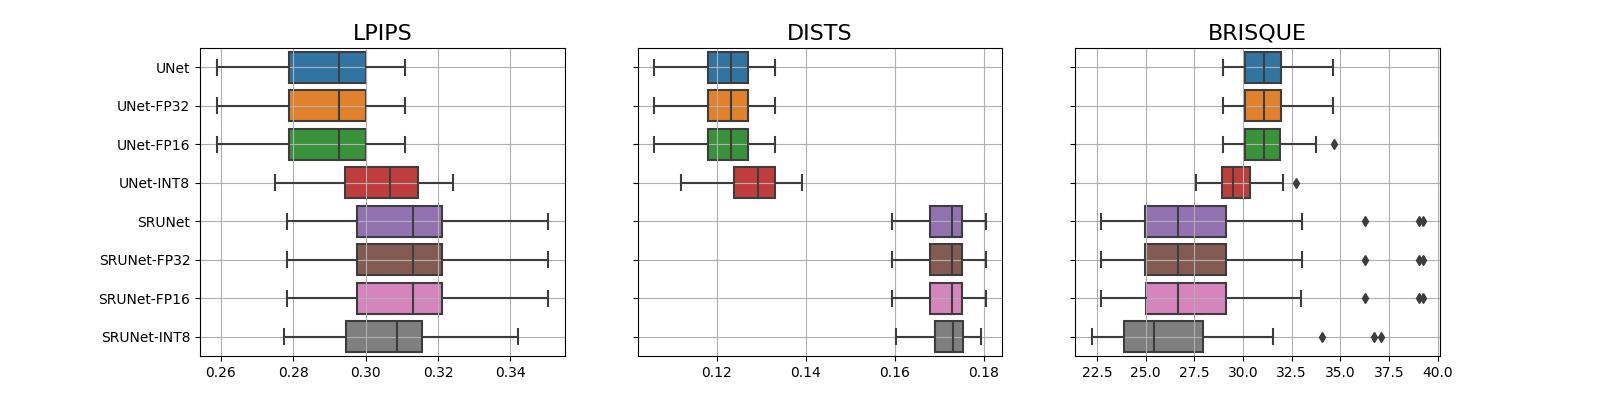
\includegraphics[width=\textwidth]{../thesis/static/boxplots_perceptual_metrics.jpg}
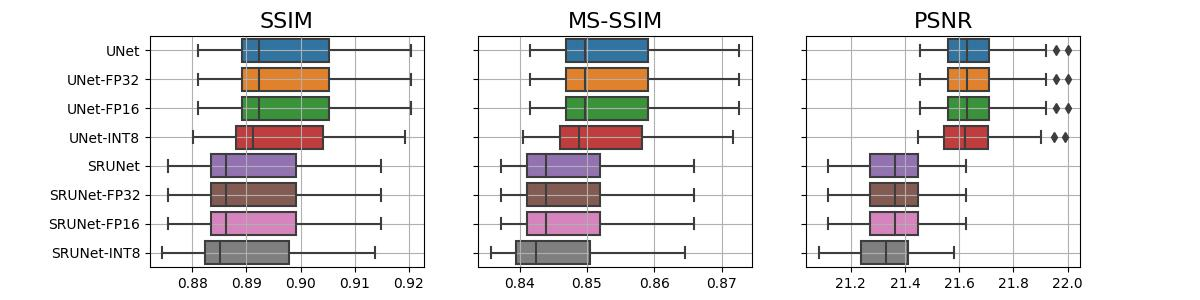
\includegraphics[width=\textwidth]{../thesis/static/boxplots_traditional_metrics.jpg}
% \caption{Perceptual Metrics}
\column{0.5\textwidth}
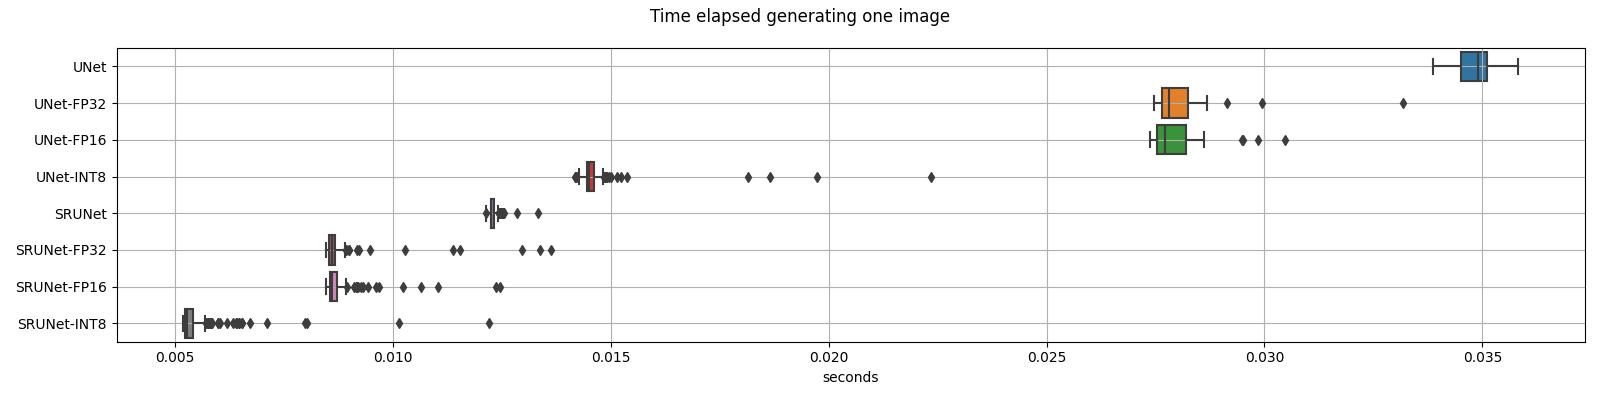
\includegraphics[width=\textwidth]{../thesis/static/boxplots_timings.jpg}
% \caption{Traditional Metrics}
\end{columns}
\end{frame}
%---------------------------------------------------------------------------------------

% %---------------------------------------------------------------------------------------
% \begin{frame}{Inference Speed and Qualitative Results}
% \begin{columns}
% \column{0.5\textwidth}
% % \caption{Inference Speed}
% % \column{0.5\textwidth}
% \includegraphics[width=\textwidth]{../thesis/static/trees-qualitative-unet.jpg}
% % \caption{Qualitative Results: Trees (UNet)}
% \end{columns}
% \end{frame}
% %---------------------------------------------------------------------------------------

%---------------------------------------------------------------------------------------
\begin{frame}{Conclusions}
\begin{itemize}
  \item Investigated post-training quantization techniques for optimizing deep learning models in super-resolution
  \item Achieved up to 2.38X speedup and 63.3\% size reduction without compromising performance
  \item Utilized TensorRT for further efficiency improvement and GPU compatibility
  \item Future research: pruning, weight sharing, model distillation, and exploring different quantization parameters
  \item Aim to stimulate advancements in optimizing deep learning models for video quality improvement
\end{itemize}
\end{frame}
%---------------------------------------------------------------------------------------

%---------------------------------------------------------------------------------------
% DO-YOU-HAVE-ANY-QUESTIONS
%---------------------------------------------------------------------------------------
\begin{frame}[c,noframenumbering]

  {\Huge \emph{Thanks for your attention!}}

  \begin{itemize}
    \item[]
    \item[]
  \end{itemize}

  \LARGE Do you have any questions?

\end{frame}
%---------------------------------------------------------------------------------------

%---------------------------------------------------------------------------------------
% BIBLIOGRAPHY
%---------------------------------------------------------------------------------------
\begingroup
\footnotesize
\begin{frame}[noframenumbering]{References}
\begin{thebibliography}{99}

% \bibitem{bib:kocher}{Kocher, P.C., 1996, August. Timing attacks on implementations of Diffie-Hellman, RSA, DSS, and other systems. In Annual International Cryptology Conference (pp. 104-113). Springer, Berlin, Heidelberg.}
% \bibitem{bib:openssl}{Brumley, D. and Boneh, D., 2005. Remote timing attacks are practical. Computer Networks, 48(5), pp.701-716.}
% \bibitem{bib:boreale}{Boreale, M., 2003. Note per il corso di Sicurezza delle Reti.}
% \bibitem{bib:montgomery}{Montgomery, P.L., 1985. Modular multiplication without trial division. Mathematics of computation, 44(170), pp.519-521.}
% \bibitem{bib:sliding}{Menezes, A.J., Van Oorschot, P.C. and Vanstone, S.A., 2018. Handbook of applied cryptography. CRC press.}
% \bibitem{bib:schindler}{Schindler, W., 2000, August. A timing attack against RSA with the chinese remainder theorem. In International Workshop on Cryptographic Hardware and Embedded Systems (pp. 109-124). Springer, Berlin, Heidelberg.}
% \bibitem{bib:coppersmith}{Coppersmith, D., 1997. Small solutions to polynomial equations, and low exponent RSA vulnerabilities. Journal of cryptology, 10(4), pp.233-260.}

\end{thebibliography}
\end{frame}
\endgroup
%---------------------------------------------------------------------------------------

\end{document}

